% MemTab IEEE manuscript. Upload this file alone, or use memtab_overleaf.zip.
% Measurement macros preserve the supplied paper/results.csv verbatim.
\documentclass[conference]{IEEEtran}
\usepackage[T1]{fontenc}
\usepackage[utf8]{inputenc}
\usepackage{cite}
\usepackage{amsmath,amssymb}
\usepackage{booktabs}
\usepackage{graphicx}
\usepackage{url}
\usepackage{tikz}
\usetikzlibrary{arrows.meta,positioning}
\usepackage{pgfplots}
\usepgfplotslibrary{groupplots}
\pgfplotsset{compat=1.18}
\usepackage[hidelinks]{hyperref}

% BEGIN EMBEDDED BIBLIOGRAPHY
\begin{filecontents*}{references.bib}
@inproceedings{reimers2019sbert,
  author = {Nils Reimers and Iryna Gurevych},
  title = {Sentence-{BERT}: Sentence Embeddings using Siamese {BERT}-Networks},
  booktitle = {Proceedings of EMNLP-IJCNLP},
  year = {2019}, pages = {3982--3992},
  doi = {10.18653/v1/D19-1410},
  url = {https://aclanthology.org/D19-1410/}
}
@inproceedings{wang2020minilm,
  author = {Wenhui Wang and Furu Wei and Li Dong and Hangbo Bao and Nan Yang and Ming Zhou},
  title = {{MiniLM}: Deep Self-Attention Distillation for Task-Agnostic Compression of Pre-Trained Transformers},
  booktitle = {Advances in Neural Information Processing Systems},
  volume = {33}, pages = {5776--5788}, year = {2020},
  url = {https://arxiv.org/abs/2002.10957}
}
@inproceedings{lewis2020rag,
  author = {Patrick Lewis and Ethan Perez and Aleksandra Piktus and Fabio Petroni and Vladimir Karpukhin and Naman Goyal and Heinrich Kuttler and Mike Lewis and Wen-tau Yih and Tim Rockt{\"a}schel and Sebastian Riedel and Douwe Kiela},
  title = {Retrieval-Augmented Generation for Knowledge-Intensive {NLP} Tasks},
  booktitle = {Advances in Neural Information Processing Systems},
  volume = {33}, pages = {9459--9474}, year = {2020},
  url = {https://arxiv.org/abs/2005.11401}
}
@inproceedings{karpukhin2020dpr,
  author = {Vladimir Karpukhin and Barlas O{\u{g}}uz and Sewon Min and Patrick Lewis and Ledell Wu and Sergey Edunov and Danqi Chen and Wen-tau Yih},
  title = {Dense Passage Retrieval for Open-Domain Question Answering},
  booktitle = {Proceedings of EMNLP},
  pages = {6769--6781}, year = {2020},
  doi = {10.18653/v1/2020.emnlp-main.550},
  url = {https://aclanthology.org/2020.emnlp-main.550/}
}
@inproceedings{haas2017wasm,
  author = {Andreas Haas and Andreas Rossberg and Derek L. Schuff and Ben L. Titzer and Michael Holman and Dan Gohman and Luke Wagner and Alon Zakai and J. F. Bastien},
  title = {Bringing the Web up to Speed with {WebAssembly}},
  booktitle = {Proceedings of ACM SIGPLAN PLDI},
  pages = {185--200}, year = {2017},
  doi = {10.1145/3062341.3062363}
}
@inproceedings{jacob2018quantization,
  author = {Benoit Jacob and Skirmantas Kligys and Bo Chen and Menglong Zhu and Matthew Tang and Andrew Howard and Hartwig Adam and Dmitry Kalenichenko},
  title = {Quantization and Training of Neural Networks for Efficient Integer-Arithmetic-Only Inference},
  booktitle = {Proceedings of IEEE CVPR},
  pages = {2704--2713}, year = {2018},
  doi = {10.1109/CVPR.2018.00286}
}
@article{jegou2011pq,
  author = {Herv{\'e} J{\'e}gou and Matthijs Douze and Cordelia Schmid},
  title = {Product Quantization for Nearest Neighbor Search},
  journal = {IEEE Transactions on Pattern Analysis and Machine Intelligence},
  volume = {33}, number = {1}, pages = {117--128}, year = {2011},
  doi = {10.1109/TPAMI.2010.57}
}
@inproceedings{charikar2002hashing,
  author = {Moses S. Charikar},
  title = {Similarity Estimation Techniques from Rounding Algorithms},
  booktitle = {Proceedings of ACM STOC},
  pages = {380--388}, year = {2002},
  doi = {10.1145/509907.509965}
}
@article{vinh2010nmi,
  author = {Nguyen Xuan Vinh and Julien Epps and James Bailey},
  title = {Information Theoretic Measures for Clusterings Comparison: Variants, Properties, Normalization and Correction for Chance},
  journal = {Journal of Machine Learning Research},
  volume = {11}, pages = {2837--2854}, year = {2010},
  url = {https://jmlr.org/papers/v11/vinh10a.html}
}
@article{shi2016edge,
  author = {Weisong Shi and Jie Cao and Quan Zhang and Youhuizi Li and Lanyu Xu},
  title = {Edge Computing: Vision and Challenges},
  journal = {IEEE Internet of Things Journal},
  volume = {3}, number = {5}, pages = {637--646}, year = {2016},
  doi = {10.1109/JIOT.2016.2579198}
}
@misc{onnxruntimeweb,
  author = {{Microsoft}}, title = {{ONNX Runtime Web}},
  howpublished = {\url{https://onnxruntime.ai/docs/tutorials/web/}},
  note = {Online documentation}
}
@misc{transformersjs,
  author = {{Hugging Face}}, title = {{Transformers.js} Documentation},
  howpublished = {\url{https://huggingface.co/docs/transformers.js/}},
  note = {Online documentation}
}
@misc{minilmcheckpoint,
  author = {{Xenova}}, title = {{all-MiniLM-L6-v2}: Model Card and {ONNX} Files},
  howpublished = {\url{https://huggingface.co/Xenova/all-MiniLM-L6-v2}},
  note = {Model identifier used by the implementation}
}
@misc{chromemv3,
  author = {{Google Chrome Developers}}, title = {The Extension Service Worker Lifecycle},
  howpublished = {\url{https://developer.chrome.com/docs/extensions/develop/concepts/service-workers/lifecycle}},
  note = {Online documentation}
}
@misc{chromeoffscreen,
  author = {{Google Chrome Developers}}, title = {The {chrome.offscreen} {API}},
  howpublished = {\url{https://developer.chrome.com/docs/extensions/reference/api/offscreen}},
  note = {Online documentation}
}
@misc{chromegrouping,
  author = {{Google Chrome Developers}}, title = {Group Tabs},
  howpublished = {\url{https://developer.chrome.com/docs/extensions/reference/api/tabs#method-group}},
  note = {Native tab-group operation used by the implementation}
}
@misc{indexeddb,
  author = {{World Wide Web Consortium}}, title = {Indexed Database {API}},
  howpublished = {\url{https://www.w3.org/TR/IndexedDB/}},
  note = {Web database specification}
}
\end{filecontents*}
% END EMBEDDED BIBLIOGRAPHY

% BEGIN CSV METRICS
\newcommand{\mDocuments}{240}
\newcommand{\mQueries}{40}
\newcommand{\mDimensions}{384}
\newcommand{\mConcurrency}{12}
\newcommand{\mInitialization}{599.5}
\newcommand{\mDocMean}{46.0412499991556}
\newcommand{\mDocMedian}{43.60000002384186}
\newcommand{\mDocTail}{62.90000003576279}
\newcommand{\mQueryMean}{15.72749999910593}
\newcommand{\mQueryMedian}{15.900000035762787}
\newcommand{\mQueryTail}{18.899999976158142}
\newcommand{\mInitialHeap}{10.534808158874512}
\newcommand{\mPeakHeap}{43.436079025268555}
\newcommand{\mThreshold}{0.45}
\newcommand{\mClusters}{38}
\newcommand{\mNMI}{0.729755834733093}
\newcommand{\mClusteringTime}{89.80000001192093}
\newcommand{\mFullTokens}{20617}
\newcommand{\mPrunedTokens}{10109}
\newcommand{\mTokenReduction}{50.96764805742834}
\newcommand{\mFloatBytes}{368640}
\newcommand{\mFloatScanMean}{0.29450000047683716}
\newcommand{\mFloatScanMedian}{0.30000001192092896}
\newcommand{\mFloatScanTail}{0.5}
\newcommand{\mFloatRecallOne}{0.13333333333333333}
\newcommand{\mFloatRecallFive}{0.6666666666666665}
\newcommand{\mFloatRecallTen}{0.9375000000000007}
\newcommand{\mFloatHitOne}{0.8000000000000004}
\newcommand{\mFloatHitFive}{0.9500000000000005}
\newcommand{\mFloatMRR}{0.8695833333333337}
\newcommand{\mIntBytes}{92160}
\newcommand{\mIntScanMean}{0.5985000002384185}
\newcommand{\mIntScanMedian}{0.5999999642372131}
\newcommand{\mIntScanTail}{1}
\newcommand{\mIntRecallOne}{0.13333333333333333}
\newcommand{\mIntRecallFive}{0.6666666666666665}
\newcommand{\mIntRecallTen}{0.9333333333333339}
\newcommand{\mIntHitOne}{0.8000000000000004}
\newcommand{\mIntHitFive}{0.9500000000000005}
\newcommand{\mIntMRR}{0.8645833333333337}
\newcommand{\mBinaryBytes}{11520}
\newcommand{\mBinaryScanMean}{0.07499999970197678}
\newcommand{\mBinaryScanMedian}{0.09999996423721313}
\newcommand{\mBinaryScanTail}{0.19999998807907104}
\newcommand{\mBinaryRecallOne}{0.10833333333333332}
\newcommand{\mBinaryRecallFive}{0.5291666666666668}
\newcommand{\mBinaryRecallTen}{0.8041666666666671}
\newcommand{\mBinaryHitOne}{0.6500000000000002}
\newcommand{\mBinaryHitFive}{0.8250000000000004}
\newcommand{\mBinaryMRR}{0.7532142857142857}
% END CSV METRICS

\newcommand{\checkpoint}{\texttt{Xenova/all-MiniLM-L6-v2}}
\definecolor{plotblue}{HTML}{4477AA}
\definecolor{plotgreen}{HTML}{228833}

% Native chart fallbacks avoid missing assets in a single-file upload.
\newcommand{\NativeTradeoffFigure}{%
\begin{tikzpicture}
\begin{groupplot}[
 group style={group size=2 by 2,horizontal sep=1cm,vertical sep=1.1cm},
 width=0.43\textwidth,height=3.3cm,
 tick label style={font=\scriptsize},label style={font=\scriptsize},
 title style={font=\scriptsize},xtick={0,1,2},
 xticklabels={Float32,Int8,Binary},xmin=-0.5,xmax=2.5,
 ymajorgrids,grid style={gray!20},axis lines*=left,
 bar width=13pt,scaled y ticks=false,
]
\nextgroupplot[title={(a) Packed vector storage},ylabel={Bytes},ymin=0]
\addplot[ybar,fill=plotblue,draw=black] coordinates
 {(0,\mFloatBytes) (1,\mIntBytes) (2,\mBinaryBytes)};
\nextgroupplot[title={(b) Warm scan and sort},ylabel={Latency (ms)},ymin=0,ymax=1.2]
\addplot[ybar,fill=plotblue,draw=black] coordinates
 {(0,\mFloatScanMedian) (1,\mIntScanMedian) (2,\mBinaryScanMedian)};
\addplot[only marks,mark=diamond*,black] coordinates
 {(0,\mFloatScanTail) (1,\mIntScanTail) (2,\mBinaryScanTail)};
\legend{P50,P95}
\nextgroupplot[title={(c) Judged Recall@5},ylabel={Recall@5},ymin=0,ymax=1]
\addplot[ybar,fill=plotgreen,draw=black] coordinates
 {(0,\mFloatRecallFive) (1,\mIntRecallFive) (2,\mBinaryRecallFive)};
\nextgroupplot[title={(d) Reciprocal-rank quality},ylabel={MRR@10},ymin=0,ymax=1]
\addplot[ybar,fill=plotgreen,draw=black] coordinates
 {(0,\mFloatMRR) (1,\mIntMRR) (2,\mBinaryMRR)};
\end{groupplot}
\end{tikzpicture}}

\newcommand{\NativeTokenFigure}{%
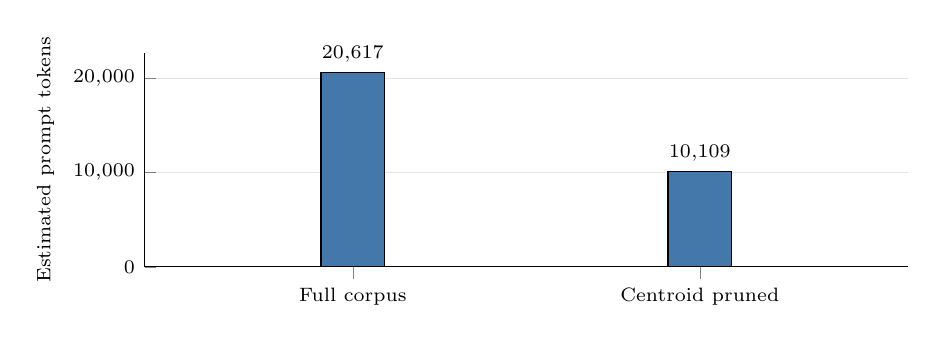
\begin{tikzpicture}
\begin{axis}[
 width=0.93\columnwidth,height=4.3cm,
 ybar,bar width=23pt,xtick={0,1},
 xticklabels={Full corpus,Centroid pruned},
 xmin=-0.6,xmax=1.6,ymin=0,
 ylabel={Estimated prompt tokens},
 tick label style={font=\scriptsize},label style={font=\scriptsize},
 ymajorgrids,grid style={gray!20},axis lines*=left,
 scaled y ticks=false,nodes near coords,
 every node near coord/.append style={font=\scriptsize},
]
\addplot[fill=plotblue,draw=black] coordinates
 {(0,\mFullTokens) (1,\mPrunedTokens)};
\end{axis}
\end{tikzpicture}}

\title{MemTab: Local Semantic Browser Memory with\\
Quantized Search and Selective Cloud Offloading}
\author{\IEEEauthorblockN{Author Name}
\IEEEauthorblockA{Department / Laboratory Name\\
Institution Name\\
City, Country\\
author@example.edu}}

\begin{document}
\maketitle

\begin{abstract}
Browser memory must retain useful page representations while operating within
the lifecycle constraints of Chrome Manifest V3 and avoiding routine disclosure
of browsing content to remote inference services. This paper presents MemTab,
a local-first extension that extracts bounded page text, runs a quantized
MiniLM encoder in a single-threaded WebAssembly offscreen document, and stores
one selected vector representation in IndexedDB. Local average-linkage
clustering selects centroid-nearest representatives for optional cloud naming
of tab groups. A synthetic workload contains \mDocuments{} documents across
eight topics and \mQueries{} judged queries. Packed-vector storage is
\mFloatBytes{}, \mIntBytes{}, and \mBinaryBytes{} bytes for Float32, Int8, and
Binary, respectively. Binary scan P95 is \mBinaryScanTail{} ms, while Int8
Recall@5 is \mIntRecallFive{}. Estimated prompt size decreases from
\mFullTokens{} to \mPrunedTokens{} tokens, a
\mTokenReduction{}\% reduction, with clustering NMI of \mNMI{}.
Fresh-engine initialization takes \mInitialization{} ms; download-cache
state is unrecorded. The evaluation separates scan latency from query
inference and reports observed JavaScript heap rather than total process RAM.
These results characterize the implemented browser pipeline on a controlled
synthetic trace, without establishing zero lexical overlap, real-world
retrieval quality, or an end-to-end latency guarantee.
\end{abstract}
\begin{IEEEkeywords}
edge computing, browser extensions, semantic retrieval, WebAssembly,
vector quantization, selective cloud offloading
\end{IEEEkeywords}

\section{Introduction}
\IEEEPARstart{B}{rowser} tabs, bookmarks, and history form a distributed personal
information collection. The browser remembers where a user navigated, but
recovering a page often requires remembering the vocabulary of its title or
address. Dense sentence representations offer a complementary retrieval path:
a conceptually related query can retrieve a page even when its title is
unfamiliar~\cite{reimers2019sbert,karpukhin2020dpr}. Applying this mechanism to
personal browsing introduces systems constraints that differ from a
server-hosted document collection.

First, useful information is encountered incrementally inside heterogeneous
web pages. An extension must extract content from partially hydrated documents,
associate it with browser metadata, and preserve it after the tab closes.
Second, Chrome Manifest V3 uses event-driven service workers whose global
state is not a durable execution context~\cite{chromemv3}. A model singleton,
an unfinished embedding queue, or an in-memory index cannot rely on the
coordinator remaining alive. Third, local computation competes with the
browser's existing workload, while cloud-only processing adds a disclosure
boundary and a network dependency. An edge--cloud design should specify which
data crosses that boundary rather than treating all page content as a default
cloud input~\cite{shi2016edge}.

MemTab addresses these constraints with an offscreen inference document,
durable page records, and a selectable compressed-vector representation.
The extension captures text from visited pages and imports title/address
metadata from bookmarks and recent history. Its local encoder creates
semantic vectors, while the command palette combines vector similarity with
lexical relevance. Workspace organization follows a separate path:
local clustering determines membership, and an optional remote language
model supplies short labels and a session brief from a reduced payload.
Users review the proposed groups before native Chrome groups are applied.

This division limits cloud dependence, but it does not imply that every
component is free of network access. Model weights and tokenizer data are
downloaded during setup and cached in the browser. Cloud naming, when enabled,
deliberately transmits selected snippets and titles. Nor does compressed
vector storage bound the entire extension footprint: page text, object
metadata, model allocations, and WebAssembly memory remain distinct costs.
An evaluation must therefore identify the boundary of each measurement.

The paper makes three concrete systems contributions:
\begin{enumerate}
 \item A lifecycle-aware browser memory pipeline that separates the Manifest
 V3 coordinator from local inference, reconstructs pending work from
 IndexedDB, and retains usable metadata while semantic indexing is unavailable.
 \item A selectable Float32, Int8, and sign-bit vector engine, evaluated with
 shared embeddings and explicit relevance judgments to expose storage,
 ranking-quality, and scan-latency tradeoffs.
 \item A local clustering and representative-selection path for optional
 cloud naming, together with an exportable benchmark that distinguishes
 inference, scan, heap, clustering, and estimated payload costs.
\end{enumerate}
These contributions concern integration and measurement. The encoder,
quantizers, and clustering family are established techniques; the paper does
not propose a new retrieval model or clustering algorithm.

\section{Background and Related Work}
\subsection{Dense Retrieval and Server-Side RAG}
Sentence-BERT maps sentences into representations that can be compared without
jointly encoding every query--document pair~\cite{reimers2019sbert}.
Dense passage retrieval applies learned representations to retrieving evidence
from document collections~\cite{karpukhin2020dpr}, while retrieval-augmented
generation conditions a generator on retrieved information~\cite{lewis2020rag}.
These approaches motivate semantic representations, but a server-side
deployment can centralize ingestion, indexing, and inference in a continuously
available backend. A browser extension must instead manage navigation events,
permissions, suspension, and a private local collection.

MemTab is not a full retrieval-augmented question-answering system. Its
retrieval interface opens matching pages rather than generating answers from
their contents. The optional generator labels tab clusters; it neither
determines vector rankings nor receives a complete browsing collection.
Consequently, this evaluation does not measure answer factuality,
generation quality, or server-side retrieval throughput.

\subsection{Cloud-Only Organization and Selective Offloading}
A cloud-only organizer can send page descriptions to a remote model and
delegate grouping and naming together. That design moves semantic inference
and membership decisions away from the browser, and the amount of submitted
text grows with the described workspace. MemTab instead fixes memberships
locally and offloads only optional naming. It preserves a provider-independent
local mode and an explicit preview before applying groups.

This architectural comparison should not be confused with an empirical
comparison against a commercial organizer. The supplied benchmark includes
neither cloud-service timings nor measured provider billing. The full-corpus
payload is a defined serialization baseline; it is not a recorded request
from another product. Estimated character-based token counts therefore support
a payload-size comparison, not a claim about a provider's cost or response
quality.

\subsection{Client-Side WebAssembly Inference}
WebAssembly provides a portable execution target for web
applications~\cite{haas2017wasm}. ONNX Runtime Web exposes browser inference
backends~\cite{onnxruntimeweb}, and Transformers.js supplies model loading,
tokenization, and pipeline interfaces~\cite{transformersjs}. MemTab uses the
\checkpoint{} checkpoint~\cite{minilmcheckpoint}, derived from the MiniLM
family of distilled transformer representations~\cite{wang2020minilm}.
The pipeline requests quantized model weights and a WebAssembly execution
device. Model-weight quantization is independent of the selectable
post-inference vector encoding.

The offscreen API supplies an extension document with web-platform facilities
while the coordinator remains a service worker~\cite{chromeoffscreen}.
This is an execution separation, not a promise of indefinite persistence.
Durable records and restart reconstruction remain necessary.

\subsection{Scalar and Binary Vector Compression}
Quantization reduces numerical representation cost at the expense of
approximation error. Quantized neural inference~\cite{jacob2018quantization}
and retrieval-vector compression address different stages of the pipeline.
Product quantization learns codebooks for vector subspaces and supports
compressed approximate distance evaluation~\cite{jegou2011pq}. MemTab does
not implement product quantization: its Int8 mode applies a fixed scalar
mapping to each normalized coordinate.

Binary hashing connects compact codes with similarity estimation under
appropriate constructions~\cite{charikar2002hashing}. MemTab stores coordinate
signs directly, without learned thresholds or random projections. Its
Hamming-based score is therefore an implementation-specific surrogate for
continuous similarity, whose usefulness must be evaluated on the workload.
The principal benefit is packed storage and word-level XOR/popcount
comparison; fidelity to the original ranking is not assumed.

\section{System Architecture}
\begin{figure*}[!t]
\centering
\resizebox{0.98\textwidth}{!}{%
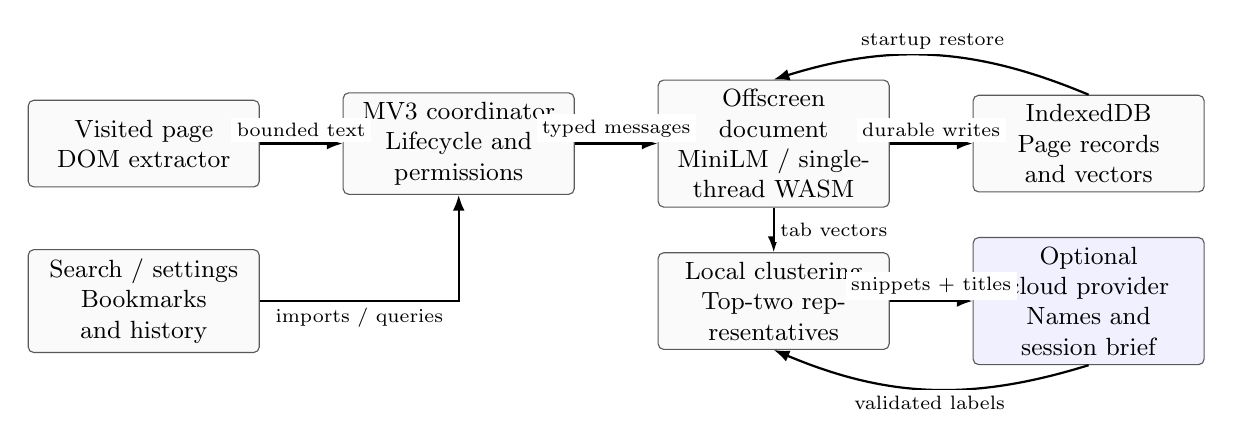
\begin{tikzpicture}[
 box/.style={draw=black!65,rounded corners=2pt,align=center,
 text width=2.7cm,minimum height=1.1cm,font=\small,fill=gray!4},
 remote/.style={box,fill=blue!6},
 arrow/.style={-{Latex[length=2mm]},thick},
 note/.style={font=\scriptsize,align=center,fill=white,inner sep=2pt},
]
\node[box] (capture) at (0,0) {Visited page\\DOM extractor};
\node[box] (worker) at (4,0) {MV3 coordinator\\Lifecycle and permissions};
\node[box] (engine) at (8,0) {Offscreen document\\MiniLM / single-thread WASM};
\node[box] (db) at (12,0) {IndexedDB\\Page records and vectors};
\node[box] (ui) at (0,-2) {Search / settings\\Bookmarks and history};
\node[box] (groups) at (8,-2) {Local clustering\\Top-two representatives};
\node[remote] (cloud) at (12,-2) {Optional cloud provider\\Names and session brief};
\draw[arrow] (capture) -- node[note,above] {bounded text} (worker);
\draw[arrow] (worker) -- node[note,above] {typed messages} (engine);
\draw[arrow] (engine) -- node[note,above] {durable writes} (db);
\draw[arrow] (db.north) to[bend right=20] node[note,above] {startup restore} (engine.north);
\draw[arrow] (ui.east) -| node[note,near start,below] {imports / queries} (worker.south);
\draw[arrow] (engine) -- node[note,right] {tab vectors} (groups);
\draw[arrow] (groups) -- node[note,above] {snippets + titles} (cloud);
\draw[arrow] (cloud.south) to[bend left=20] node[note,below] {validated labels} (groups.south);
\end{tikzpicture}}
\caption{Implemented data paths. The coordinator routes local capture, imports,
and search to the offscreen engine. Workspace membership is determined
locally; the optional remote provider receives a reduced naming payload.
Native group application follows user review.}
\label{fig:architecture}
\end{figure*}

\subsection{Heuristic DOM Boilerplate Pruning}
A top-level content script runs on HTTP(S) pages and observes DOM changes.
After an initial hydration delay, it clones the body and removes scripts,
styles, navigation, footers, sidebars, forms, inputs, editable regions, and
selected advertisement and cookie-banner selectors. It prefers an article,
main element, or main-role region, falling back to the clone. Heading text is
combined with traversed text nodes, whitespace is collapsed, and captured
text is capped at 1,200 characters. The script deduplicates unchanged content
and defers capture while the document is hidden.

This procedure is a bounded heuristic rather than a complete article parser.
It may retain boilerplate not covered by the selectors or omit material in
embedded frames and dynamically protected interfaces. The bound limits input
and retained-text cost but can discard relevant material late in a document.
The encoder receives the title and stored text through a separately bounded
input string.

Imported bookmarks, history, and initial open-tab synchronization create
metadata records without fetching old pages. A later visit can replace
metadata text with captured content, while a later import cannot overwrite
already captured article text. Canonical HTTP(S) addresses merge duplicate
records and strip fragments. Source tags retain bookmark and history
membership; open-tab status is queried from Chrome rather than preserved as a
potentially stale tab identifier.

\subsection{Offscreen Execution and Mutex Lifecycle}
The coordinator checks \texttt{chrome.offscreen.hasDocument()} before forwarding
engine operations. A shared creation promise serializes concurrent creation
attempts; a separate configuration promise initializes settings in the engine.
The document is created with the \texttt{WORKERS} reason. The offscreen context
uses runtime messaging and web APIs rather than treating it as a
general-purpose extension API context.

The encoder pipeline is loaded through a singleton promise. The configuration
selects \texttt{dtype: q8}, \texttt{device: wasm}, one WASM thread, and disabled
proxy execution. Mean pooling and normalization produce a
\mDimensions{}-dimensional vector. Executable runtime files are packaged
with the extension, and the module factory is referenced directly. The
library's blob-based WASM cache is disabled to respect the extension's
content-security policy. Model data, by contrast, use the browser cache after
the user enables semantic search.

Inference requests share a promise chain. Background indexing processes one
document at a time, allowing query work to enter between documents without
duplicating the model. The memory engine mirrors IndexedDB records in a
JavaScript map~\cite{indexeddb}. Missing vectors, changed text signatures, and
changed precision identify pending work after restoration. A generation check
prevents an in-flight embedding from restoring a page after a clear operation.
Periodic coordinator alarms resume pending indexing.

The selected vector encoding is stored with each record; all encodings are not
retained simultaneously in the production index. Rebuilding after a precision
change re-embeds saved text. Domain exclusions delete matching memories, and
browser history and bookmark removal update source membership. These behaviors
bound state inconsistency but have not been evaluated under forced browser
crashes or prolonged memory pressure.

\subsection{Quantized Vector Engine and Scan Boundary}
For normalized encoder output $x\in\mathbb{R}^{d}$, where
$d=\mDimensions$, Float32 retains the original coordinates. Int8 applies
\begin{equation}
 q_i=\operatorname{round}\!\left(127\,
       \operatorname{clip}(x_i,-1,1)\right).
 \label{eq:int8}
\end{equation}
The Int8 similarity function computes cosine similarity using the quantized
coordinates and their norms, rather than assuming quantization preserves
unit length. Float32 uses the same cosine function on floating-point
coordinates. The weights of the neural model remain q8 in all vector modes.

Binary encoding maps a coordinate to a sign bit,
$b_i=\mathbf{1}[x_i\geq0]$, and packs bits into unsigned machine words.
The implementation uses XOR and a SWAR population-count sequence to compute
\begin{equation}
 s_{\mathrm{bin}}(a,b)=1-
 \frac{\operatorname{popcount}(a\mathbin{\mathrm{XOR}}b)}{d}.
 \label{eq:binary}
\end{equation}
The encoder dimension aligns with the word packing; the utility also masks
unused bits for partial terminal words. Packed payload cost follows from
coordinate width, while JavaScript object and database overhead are additional.

Retrieval scans the map and sorts candidates. The scoring phase has linear
dependence on collection size; sorting contributes a separate
$O(N\log N)$ term in the implementation. A query embedding is compressed once
for each representation encountered, accommodating records in transition
between modes. The production ranking uses
$s_{\mathrm{hybrid}}=0.85s_{\mathrm{semantic}}+0.15s_{\mathrm{lexical}}$.
When the model is unavailable, keyword search remains usable. Repeated query
embeddings are cached within the offscreen engine.

The benchmark measures semantic scan-and-sort latency over an isolated
collection, excluding query embedding. It does not time the production hybrid
path, Chrome tab-state lookup, message serialization, rendering, or queue
waiting. A small scan measurement is consequently not a bound on the complete
command-palette response.

\subsection{Agglomerative Clustering and Top-Two Cloud Pruning}
Workspace organization considers unpinned web tabs in the selected window.
Available non-binary vectors are normalized for clustering; missing, stale,
or binary records can be re-embedded from their stored text or metadata.
The coordinator limits the organizer's input size, while the benchmark
clusters the synthetic corpus separately.

Average-linkage agglomeration initializes pairwise cosine distances and
merges the closest eligible pair until no distance is at most
$\tau=\mThreshold$. If $A$ and $B$ merge, distances to another cluster $C$
are updated by
\begin{equation}
 D(A\cup B,C)=
 \frac{|A|D(A,C)+|B|D(B,C)}{|A|+|B|}.
 \label{eq:linkage}
\end{equation}
The distance matrix requires quadratic space. Repeated searches for the
closest active pair make this implementation cubic in the worst case; the
weighted update avoids recomputing every member pair but does not remove that
search cost.

For a non-singleton cluster, the implementation normalizes the sum of member
vectors and selects the two members most similar to that centroid. These are
centroid-nearest, medoid-style representatives: the code ranks members by
centroid similarity rather than solving a separate multi-medoid objective.
Singleton clusters are omitted from the remote naming payload.

Each transmitted cluster includes representative titles, bounded snippets,
and shorter titles for remaining members. No explicit URL field is added;
however, imported metadata can contain an address inside its text, so field
omission does not establish URL redaction. When cloud naming is enabled, a
Gemini or OpenAI-compatible endpoint returns group labels and a session brief.
Response validation accepts labels for known cluster identifiers and
constrains colors and title length. Group membership remains local.

The proposed groups are stored as a preview. Before native grouping, the
coordinator rechecks each tab's address, window, and eligibility, skipping
closed, navigated, or pinned tabs~\cite{chromegrouping}. The architecture reduces
the amount of text submitted for naming but does not anonymize that text or
provide a formal privacy guarantee. Provider keys are locally stored settings,
not encrypted secrets.

\section{Experimental Methodology}
\subsection{Recorded Environment and Scope}
The authoritative input is the supplied \texttt{results.csv}, copied unchanged
to the paper directory. Its timestamp is
\texttt{2026-11-16T09:29:32.208Z}. The recorded user agent identifies
Windows NT on a 64-bit platform and Chrome/157.0.0.0. The browser reports
\mConcurrency{} logical hardware-concurrency slots; this does not establish the
physical core count. The encoder device is recorded as single-thread WASM,
with the q8 checkpoint identified in Section III.

The project brief targets an 8\,GB laptop, but the export records neither
physical RAM nor the CPU model. We therefore treat that capacity as a design
target, not a verified experimental hardware specification. Likewise,
browser flags, power state, cache residency, and operating-system load are
unrecorded. These gaps limit claims about cross-machine reproducibility.

The evaluated run records an unloaded engine model before initialization.
That condition identifies a fresh pipeline instance, but not an empty
download cache. The report supplies a single initialization observation and
aggregated inference distributions. It does not supply a repeated cold/warm
startup experiment, independent sessions, or confidence intervals.

\subsection{Synthetic Trace and Relevance Judgments}
The dataset contains \mDocuments{} documents in eight categories:
systems programming, model quantization, web architecture, personal finance,
cooking and nutrition, motorsport engineering, cloud operations, and linear
algebra. Each category has five retrieval intents, with six document variants
per intent. Queries describe these intents in paraphrased language, and each
of the \mQueries{} queries has six explicitly relevant document identifiers.
The category labels support a separate clustering evaluation.

The specification proposes zero-keyword-overlap queries, but the generator
does not enforce that property. For example, a systems query refers to a
\emph{native program} and a relevant document also contains \emph{native}.
We describe the actual queries as paraphrases, not zero-overlap queries.
The reuse of intent descriptions and variant templates further simplifies the
workload relative to unrelated pages collected from real browsing sessions.

Documents are embedded sequentially from title plus snippet. Queries are
embedded afterward. All representation modes share these continuous
embeddings and relevance judgments, providing a controlled representation
ablation. The benchmark does not run the DOM extractor on live sites or
measure insertion into the production IndexedDB index.

\subsection{Timing, Storage, and Retrieval Metrics}
Model initialization is timed separately from document and query inference.
For each query and mode, the runner computes an untimed warm-up ranking and
then collects five timed scan-and-sort repetitions. P50 and P95 use
nearest-rank order statistics over pooled observations. These measurements
include candidate construction and sorting; they exclude query compression
performed before the timed region, model inference, extension messaging,
production filters, and interface work.

Let $G_q$ be the relevant-document set and $R_q^{(K)}$ the top-$K$ ranking.
The runner computes
\begin{equation}
 \operatorname{Recall@}K=
 \frac{1}{|Q|}\sum_{q\in Q}
 \frac{|G_q\cap R_q^{(K)}|}{|G_q|}.
 \label{eq:recall}
\end{equation}
Hit@$K$ is the fraction of queries having any relevant result in that prefix.
MRR@10 averages the reciprocal rank of the first relevant result within the
rank cutoff, assigning zero if none occurs. Because every query has six
relevant documents, perfect Recall@1 is $1/6$, not unity. This distinction
prevents interpreting a low Recall@1 ratio as the complement of top-result
accuracy.

Storage is the sum of packed typed-array byte lengths. It excludes text,
record metadata, database structures, model weights, and runtime allocations.
Figures convert bytes to KiB only for plotting; tabulated values preserve the
CSV's byte strings. Every reported measurement in the text and tables expands
from a raw CSV macro without rounding. Extra decimal digits reflect the
export format and do not imply timer or measurement accuracy.

\subsection{Clustering, Heap, and Token Accounting}
Clustering uses the continuous document vectors and the implemented linkage
threshold. Predicted cluster identifiers are compared with the topic labels
using arithmetic-normalized mutual information~\cite{vinh2010nmi}:
\begin{equation}
 \operatorname{NMI}(L,C)=
 \frac{2I(L;C)}{H(L)+H(C)}.
 \label{eq:nmi}
\end{equation}
The code separately handles degenerate entropy cases. The clustering count
includes singleton clusters, whereas the pruned cloud payload excludes them.

Observed heap uses \texttt{performance.memory.usedJSHeapSize}, sampled
periodically and after completed work. Initial heap is observed before model
initialization; the periodic sampler begins after initialization. Thus the
reported maximum can miss a transient loading peak. It can also omit native
and WebAssembly memory and includes any preexisting engine allocations.
The CSV's MB label corresponds to bytes divided by a binary megabyte in the
runner. We retain the reported unit while identifying its calculation.

The full-payload baseline serializes every document's title and snippet.
The pruned payload serializes cluster identifiers, selected snippets, and
remaining titles with the same bounds used by the naming path. The estimator
is $T=\lceil |P|/4\rceil$ for serialized payload length $|P|$, with reduction
$100(1-T_{\mathrm{pruned}}/T_{\mathrm{full}})$. It is a character-based
approximation, omits fixed prompting overhead, and is not a provider tokenizer
or billing measurement.

\section{Evaluation and Representation Ablation}
\begin{table*}[!t]
\caption{Packed Vector Storage and Warm Scan-and-Sort Latency. Values Are Raw CSV Strings; Latencies Are in Milliseconds.}
\label{tab:scans}
\centering
\small
\setlength{\tabcolsep}{6pt}
\begin{tabular}{lrrrr}
\toprule
Representation & Packed bytes & Mean scan & P50 scan & P95 scan\\
\midrule
Float32 & \mFloatBytes & \mFloatScanMean & \mFloatScanMedian & \mFloatScanTail\\
Int8 & \mIntBytes & \mIntScanMean & \mIntScanMedian & \mIntScanTail\\
Binary & \mBinaryBytes & \mBinaryScanMean & \mBinaryScanMedian & \mBinaryScanTail\\
\bottomrule
\end{tabular}
\end{table*}

\begin{table*}[!t]
\caption{Judged Retrieval Quality with Shared Embeddings. All Values Are Ratios Preserved Verbatim from the CSV.}
\label{tab:quality}
\centering
\footnotesize
\setlength{\tabcolsep}{4pt}
\begin{tabular}{lrrrrr}
\toprule
Representation & Recall@1 & Recall@5 & Recall@10 & Hit@1 & MRR@10\\
\midrule
Float32 & \mFloatRecallOne & \mFloatRecallFive & \mFloatRecallTen & \mFloatHitOne & \mFloatMRR\\
Int8 & \mIntRecallOne & \mIntRecallFive & \mIntRecallTen & \mIntHitOne & \mIntMRR\\
Binary & \mBinaryRecallOne & \mBinaryRecallFive & \mBinaryRecallTen & \mBinaryHitOne & \mBinaryMRR\\
\bottomrule
\end{tabular}
\end{table*}

\begin{figure*}[!t]
\centering
\IfFileExists{fig_quantization_tradeoff.pdf}
 {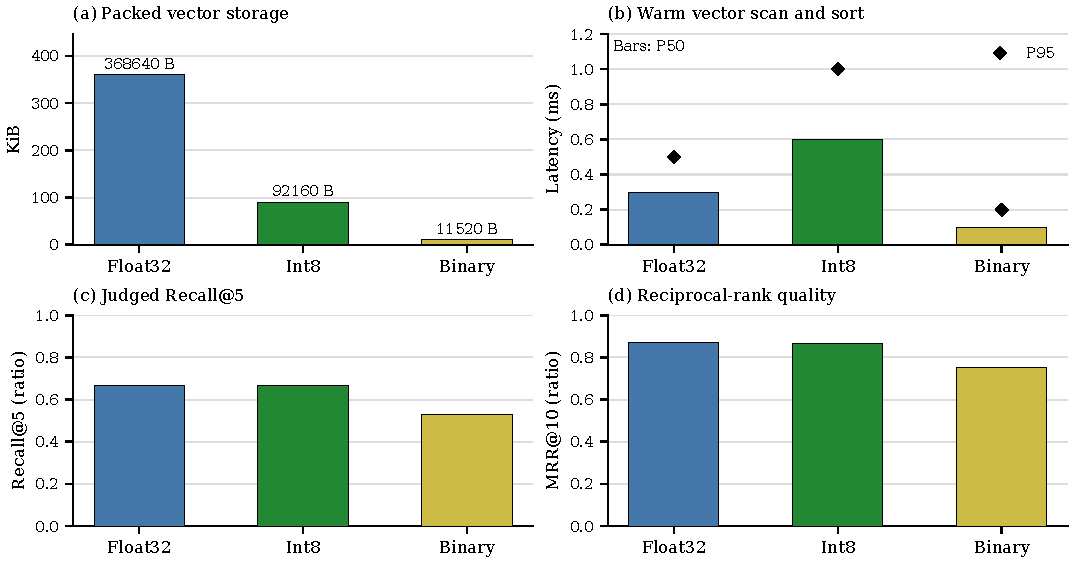
\includegraphics[width=\textwidth]{fig_quantization_tradeoff.pdf}}
 {\NativeTradeoffFigure}
\caption{Representation tradeoffs on the supplied synthetic run. Storage
uses packed-vector bytes (the generated PDF converts these to KiB); scan bars
show P50 and diamonds show P95. Recall@5 and MRR@10 use the same query judgments
and encoder outputs for every mode. Model and metadata memory are excluded
from the storage panel.}
\label{fig:tradeoff}
\end{figure*}

\subsection{Storage and Ranking-Quality Tradeoffs}
Tables~\ref{tab:scans} and~\ref{tab:quality} report the representation ablation;
Fig.~\ref{fig:tradeoff} visualizes its measured tradeoffs. Float32 stores
\mFloatBytes{} bytes, Int8 stores \mIntBytes{} bytes, and Binary stores
\mBinaryBytes{} bytes. These amounts agree with the coordinate widths and
packing rules of the implementation. They describe the isolated vector
payload, not a complete persistent index.

Float32 and Int8 have the same Recall@5,
\mFloatRecallFive{}, and the same Hit@1,
\mFloatHitOne{}, on this workload. Their rankings are not identical:
MRR@10 is \mFloatMRR{} for Float32 and \mIntMRR{} for Int8, while Recall@10
is \mFloatRecallTen{} and \mIntRecallTen{}, respectively.
The scalar encoding therefore preserves the observed short-prefix relevance
coverage while introducing smaller differences in rank placement and longer
prefix coverage.

Binary has Recall@5 of \mBinaryRecallFive{} and MRR@10 of
\mBinaryMRR{}. Its Hit@1 is \mBinaryHitOne{}, and its Recall@10 is
\mBinaryRecallTen{}. Removing coordinate magnitudes changes the neighborhood
ordering enough to reduce all of these measured quality indicators. The
results favor Binary where the smallest stored vectors and short scans are
more important than this loss in retrieval quality; they do not show that
sign codes preserve continuous-vector accuracy.

These observations define a multidimensional tradeoff rather than a single
universally preferable encoding. Int8 uses less vector storage than Float32
and remains close in measured quality, but Float32 has lower scan latency in
this run. Binary has the smallest payload and lowest scan latency, together
with the lowest measured quality. Selection depends on storage and ranking
requirements. The default Int8 configuration is a design choice rather than
an empirically optimal operating point for every browser collection.

\subsection{Warm Scans and the End-to-End Boundary}
Float32 scan P50 is \mFloatScanMedian{} ms and P95 is
\mFloatScanTail{} ms. Int8 scan P50 is \mIntScanMedian{} ms and P95 is
\mIntScanTail{} ms. Binary scan P50 is \mBinaryScanMedian{} ms and P95 is
\mBinaryScanTail{} ms. Every measured scan tail lies below the specification's
interactive scan target on this collection, but the export cannot support a
claim about larger browsing indexes.

Int8 does not automatically accelerate the scan relative to Float32.
Both modes execute cosine arithmetic in JavaScript and recompute norms;
the integer representation is not dispatched to a specialized SIMD kernel.
Storage compression alone is therefore insufficient to predict processing
speed. Binary comparisons instead exploit packed words and population count,
which is consistent with their lower measured scan cost. This interpretation
describes the code path and run; it is not an instruction-level profiling
result.

Query inference mean is \mQueryMean{} ms and P95 is \mQueryTail{} ms.
It represents a larger component than the scan measurements for this trace.
The relevant command-palette cost is conceptually
\begin{equation}
 t_{\mathrm{response}} =
 t_{\mathrm{queue}}+t_{\mathrm{embed}}+t_{\mathrm{scan}}
 +t_{\mathrm{IPC}}+t_{\mathrm{filter}}+t_{\mathrm{UI}}.
 \label{eq:latency}
\end{equation}
Only selected components are observed by this benchmark. Summing their
separately aggregated quantiles would not yield the response-time quantile.
No full-pipeline timing distribution is claimed.

\begin{table}[!t]
\caption{Initialization, Inference, and Observed Heap from the Supplied Run. Raw Values Preserve the CSV Precision.}
\label{tab:runtime}
\centering
\footnotesize
\setlength{\tabcolsep}{3pt}
\begin{tabular}{@{}lr@{}}
\toprule
Metric & Recorded value\\
\midrule
Fresh-engine initialization (ms) & \mInitialization\\
Document inference mean (ms) & \mDocMean\\
Document inference P50 (ms) & \mDocMedian\\
Document inference P95 (ms) & \mDocTail\\
Query inference mean (ms) & \mQueryMean\\
Query inference P50 (ms) & \mQueryMedian\\
Query inference P95 (ms) & \mQueryTail\\
Initial JS heap (reported MB) & \mInitialHeap\\
Peak observed JS heap (reported MB) & \mPeakHeap\\
\bottomrule
\end{tabular}
\end{table}

\subsection{Fresh Initialization, Inference, and Heap}
Table~\ref{tab:runtime} reports the initialization and inference observations.
The model is recorded as not already loaded, and initialization takes
\mInitialization{} ms. This value can include loading cached assets and
creating runtime state; the export does not identify download-cache residency
or decompose these phases. It must not be compared with an invented warm
startup number or interpreted as a network download measurement.

Document inference mean is \mDocMean{} ms, with P50
\mDocMedian{} ms and P95 \mDocTail{} ms. Query inference follows the document
phase and uses shorter paraphrase inputs; its lower measured duration cannot
be attributed exclusively to runtime warming. Input length and workload
order are confounding factors. The sequential pipeline bounds concurrent
inference work, but no throughput comparison with multi-threaded WASM or
WebGPU is present.

Initial observed JavaScript heap is \mInitialHeap{} reported MB and peak
observed heap is \mPeakHeap{} reported MB. The latter is larger than the
packed vector payload in every mode. Moreover, the benchmark retains the
continuous document and query embeddings while constructing each compressed
evaluation index. It is not a mode-isolated process-memory ablation.
These samples neither establish an extension-wide memory bound nor verify
operation under an 8\,GB physical-RAM configuration.

\subsection{Clustering and Estimated Cloud Payload}
\begin{figure}[!t]
\centering
\IfFileExists{fig_token_compression.pdf}
 {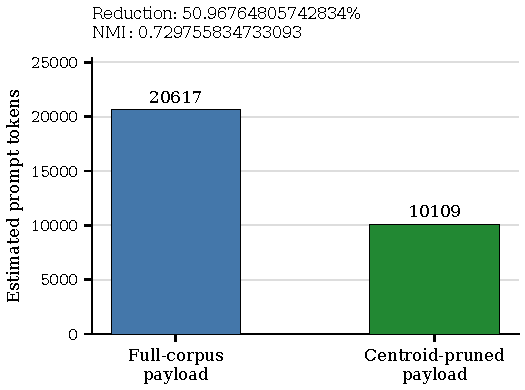
\includegraphics[width=\columnwidth]{fig_token_compression.pdf}}
 {\NativeTokenFigure}
\caption{Estimated naming payload decreases from \mFullTokens{} to
\mPrunedTokens{} tokens, a \mTokenReduction{}\% reduction.
Clustering NMI is \mNMI{}. Counts use serialized character length rather than a
provider tokenizer and omit fixed prompt overhead.}
\label{fig:tokens}
\end{figure}

At threshold \mThreshold{}, the benchmark produces \mClusters{} clusters in
\mClusteringTime{} ms, with NMI \mNMI{} against the topic labels.
The partition contains more clusters than the ground-truth topic inventory.
That outcome is consistent with narrower retrieval intents within topics and
does not establish that the organizer should create one group per topic.
NMI describes agreement with the chosen labels, not human satisfaction with
tab group membership.

The full serialization has \mFullTokens{} estimated tokens; the pruned
serialization has \mPrunedTokens{}, yielding \mTokenReduction{}\% reduction
as shown in Fig.~\ref{fig:tokens}. Retaining remaining titles and having many
clusters limits how much representative selection can shrink the payload.
This measured result replaces the more aggressive savings goal in the project
specification rather than confirming it.

The baseline already uses short synthetic snippets, not full live HTML pages.
The numerator also benefits from singleton omission and title/snippet length
bounds. The export does not isolate the contribution of representative
selection from those other pruning choices. There is no measured remote
response quality, cloud latency, or billing result. The supported conclusion
is that this implemented serialization submits a smaller estimated naming
payload while keeping membership computation local.

\section{Limitations and Future Work}
\subsection{Workload and Measurement Validity}
The synthetic collection repeats intent descriptions and document templates,
and lexical overlap is not eliminated. A natural-browsing evaluation should
include independently collected documents, harder cross-topic distractors,
human relevance judgments, and a measured lexical baseline. Without that
baseline, the current results do not quantify improvement over the extension's
keyword search or justify interpreting every hit as semantic generalization.

The supplied evidence is one exported run. The timer's decimal representation
does not substitute for independent repetitions, uncertainty estimates, or
controlled machine state. The CPU model, physical RAM, cache state, and power
settings should be recorded in future exports. Scaling tests should measure
the production map, IndexedDB restoration, message payloads, and end-to-end
query latency while indexing competes with foreground browsing.

\subsection{Single-Thread Throughput and Memory}
Sequential WASM inference limits concurrent work and avoids model duplication,
but it can delay an uncached query behind an ongoing document inference.
Repeated-query caching helps only when the same text recurs; it cannot be
treated as a universal query-speed improvement. Explicit query prioritization
and adaptive indexing backpressure are candidate extensions.

WebGPU acceleration is a future comparison, not an evaluated feature.
Its potential inference benefit must be assessed alongside device support,
initialization, transfer overhead, memory, and numerical consistency. Likewise,
observed JavaScript heap should be complemented with process-level and
WASM-aware memory instrumentation. Representation changes currently require
re-embedding stored text; evaluating alternative migration strategies would
separate inference cost from storage savings.

\subsection{Clustering Sensitivity and Offloading Quality}
Only the implemented linkage threshold is evaluated. A threshold sweep could
measure group fragmentation, singleton frequency, NMI, payload size, and
label usefulness. The present quadratic distance matrix and repeated closest
pair search also constrain large workspaces. Incremental clustering or a
more efficient nearest-pair data structure would require separate quality
and lifecycle evaluation.

Representative naming should be tested with actual providers using measured
tokenizers, label quality judgments, and controlled prompt templates.
Centroid-nearest snippets may fail to represent minority themes in a cluster.
Keeping all remaining titles partially addresses that loss while increasing
payload size. A balanced coverage selector and explicit redaction of addresses
inside metadata are possible improvements; neither is established here.

\subsection{Capture Coverage and Durable Operation}
Bounded DOM text can omit the part of an article that a user later remembers.
Metadata-only imports cannot recover historical contents that were never
captured. An optional user-triggered retrieval mechanism would introduce
network, authentication, and extraction considerations distinct from passive
capture. Current state is isolated to the Chrome profile and does not provide
cross-profile index transfer.

The lifecycle design preserves records and reconstructs missing work, but
controlled suspension, restart, duplicate-creation, and storage-failure tests
are needed for reliability claims. Offscreen execution reduces dependence on
service-worker globals; it does not make volatile state durable. The
interaction between metadata updates, deletion events, precision migration,
and inference deserves stress testing beyond functional behavior.

\section{Conclusion}
MemTab implements local semantic browser memory with a lifecycle-aware
offscreen encoder, durable records, selectable vector compression, and
optional representative-only cloud naming. The supplied run establishes
packed-storage and ranking tradeoffs across Float32, Int8, and Binary on a
judged synthetic collection. Local clustering reduces the estimated naming
payload from \mFullTokens{} to \mPrunedTokens{} tokens while leaving membership
decisions in the browser.

The principal systems lesson is to preserve measurement boundaries. Vector
scan latency is separate from query inference and interface response;
packed bytes are separate from total runtime memory; fresh model
initialization is separate from a cold download; and estimated payload tokens
are separate from cloud billing or label quality. Within those boundaries,
the prototype and exported measurements provide a reproducible basis for
broader browsing workloads, hardware-aware evaluation, and more selective
offloading policies.

\bibliographystyle{IEEEtran}
\bibliography{references}
\end{document}
